\documentclass{ctexart}
\usepackage{amsmath}
\usepackage{graphicx} % Required for inserting images
\usepackage{lipsum}
\usepackage{geometry}
\usepackage{fancyhdr}
\usepackage{lastpage}
\usepackage{placeins}
\usepackage{subcaption}
\usepackage{float} 
\usepackage{amsthm}
\usepackage{amssymb}
\usepackage{array}
\usepackage{booktabs}
\usepackage{tabularx}\usepackage{tabularx}
\usepackage{booktabs, longtable}
\newcommand{\keywords}[1]{\par\noindent\textbf{关键词：} #1}
\renewenvironment{abstract}
 {\par\large\begin{center}\textbf{\large\abstractname}\end{center}\par\noindent\ignorespaces}
 {\par}
\geometry{left=2.5cm,right=2.5cm,top=2cm,bottom=2cm}
\pagestyle{fancy}
\fancyhf{}

\rhead{ }
\cfoot{第 \thepage 页 （共 \pageref{LastPage} 页）}

\title{题目}
\author{曹建宇 \and 李正阳 \and 朱睿杰}
\date{\today}
\newtheorem{theorem}{定理}[subsection]   % 定理按节编号
\newtheorem{lemma}[theorem]{引理}     % 引理与定理共用计数器
\newtheorem{definition}{定义}[subsection]   % 定义按节编号
\begin{document}
\maketitle 
\begin{abstract}  % 摘要
这是一段摘要
\end{abstract}
\keywords{关键词1，关键词2，关键词3}  % 关键词
\newpage

\tableofcontents
\newpage
\section{问题重述} 
\subsection{问题背景}
在现代防空作战中，空地导弹凭借高精度、高速度对地面重要目标构成严重威胁。而烟幕干扰作为一种软防护措施，通过化学燃烧或爆炸分散形成烟幕或气溶胶云团在来袭导弹视线上形成遮蔽云团，可有效干扰敌方导弹，具有低成本高收益的特点，逐渐成为现代军事中防空的主流选择之一。而无人机的发展，使得烟幕弹的投放范围更加广阔，从而使得精准投放烟幕弹以达到最大遮蔽效果成为可能。

然而，无人机飞行的方向和速度，以及烟幕弹应在何处投放、应当延迟几秒起爆，极大影响最终的遮蔽效果。实际作战中，烟幕弹的下降、敌方导弹的高速移动等，使得实际的遮蔽时间非常短暂。如何通过优化，确定无人机的移动方向、移动速度以及烟幕弹投放地点、延迟起爆时间，以达到遮蔽效果的最大化，成为军事专家必须研究的课题。
\subsection{问题提出}
现已知真目标和假目标的位置和形状，三枚来袭导弹和五架无人机的坐标，以及一些运动参数，本文需要通过数学建模解决以下问题：

\textbf{问题一：}针对单架无人机，已知其运动方向、投放地点和延迟起爆时间，通过建立模型确定其仅投掷一枚烟幕弹，对一运动方向、速度固定的导弹的遮挡效果。

\textbf{问题二：}针对单架无人机，同样研究其投掷一枚烟幕弹的情形，对其飞行方向、飞行速度、烟幕干扰弹投放点、烟幕干扰弹起爆点进行优化，使得遮蔽时间最长。

\textbf{问题三：}针对单架无人机可投放多枚烟幕弹的情形，通过优化，使得其对单枚导弹的遮蔽时间最长。

\textbf{问题四：}不溶于问题三一机多弹的情形，考察三架无人机，各投放一枚烟幕弹，通过三架无人机在三维空间中的配合协调实现对于导弹的最佳屏蔽效果。

\textbf{问题五：}将问题推广到三架无人机、每架无人机最多投放三枚的情形，需要同时解决任务分配（哪架无人机干扰哪一枚导弹）和资源调度（各飞机投几枚，何时投，何时起爆）的问题。
\section{问题分析}
\subsection{问题一}
问题一是基础情况，要求计算在给定参数下烟幕干扰弹对导弹M1的有效遮蔽时长。首先可以利用题目给定的参数算出烟幕弹起爆时刻烟幕弹和导弹的位置作为后续模型的初值，之后需要根据空间几何的知识找到满足使有效遮挡这一要求成立的几何关系，最后就可以根据初值和该几何关系从起爆时刻进行变步长搜索找出满足有效遮挡的时间范围。
\subsection{问题二}
问题二不同于问题一在给定的参数下求解，而是需要延用问题一的分析，把无人机航向速度、烟幕弹投放、引爆时间四个参数作为决策变量，以最大化有效遮挡时间作为目标函数建立单机单弹情况下的策略优化模型，在满足一些物理约束、运动学约束、边界条件的情况下求解出烟幕弹的最优投放策略。
\subsection{问题三}
问题三基于问题二的优化模型，需协调多枚烟幕弹的投放与起爆时序，避免时间重叠或遗漏，通过时序优化与协同控制延长总有效遮蔽时间。由于三枚烟幕弹是由同一无人机发射，其在空间上位置相差不远，考虑有效遮挡时，可能会存在单个云团不能有效遮挡，而多个云团在时间上交替覆盖时形成连续有效遮挡的情况。
\subsection{问题四}
问题四是多机单弹拦截同一目标的情况，与问题三的单机多弹模式不同，问题四的核心在于多无人机之间的空间协同和时间协调，这里不需要考虑投弹时间间隔，但是三枚烟幕弹爆炸产生的云团应该避免在空间上过度重叠，同时时间上要保持连续。这需要建立多烟幕弹协同遮蔽的判定模型，分析多个云团在空间上的遮蔽效果叠加关系，在考虑各无人机独立决策的前提下，通过协同目标函数确保整体遮蔽效果最大化。
\subsection{问题五}
问题五是最一般化的情形，涉及5架无人机、每架至多3枚烟幕弹，同时对抗3枚来袭导弹。该问题的复杂度显著增加，需同时处理多机、多弹、多目标的分配与协同问题。核心难点在于：一方面要为每枚导弹分配合适的烟幕弹资源，另一方面要使得所有导弹在同一时刻均被至少一个云团遮蔽的时间区间尽可能长。决策变量包括各无人机的飞行方向与速度、每枚弹的投放时机和起爆延迟，以及弹与弹之间的分配关系。这属于混合整数非线性规划问题，需要建立统一的遮蔽时间并集（针对单目标）或交集（针对多目标同时遮蔽）的目标函数，并采用启发式优化算法求解全局较优的投放策略。
\section{模型假设}
\begin{enumerate}
    \item 为简化研究，我们仅研究无风情况的遮蔽，不考虑空气阻力对运动的影响。
    \item 导弹、无人机、烟幕弹、假目标均视为质点进行运动学研究。
    \item 烟幕弹起爆后瞬时膨胀成一个半径为$10m$的球，并且在有效持续时间$(20s)$内不扩散，烟雾遮蔽能力不变。
\end{enumerate}
\section{符号说明}
\begin{longtable}{@{} p{2.8cm} p{6.5cm} p{1.8cm} @{}}
% ========== 第一页的表头 ==========
\caption{导弹与烟幕弹相关符号定义}
\label{tab:symbols} \\
\toprule
\textbf{符号} & \textbf{含义} & \textbf{单位} \\
\midrule
\endfirsthead


\multicolumn{3}{c}{接上页} \\
\toprule
\textbf{符号} & \textbf{含义} & \textbf{单位} \\
\midrule
\endhead


\bottomrule
\multicolumn{3}{r}{续下页} \\
\endfoot


\bottomrule
\endlastfoot


$O_d$          & 假目标位置（原点）                                 & m \\
$O_1$          & 真目标底面圆心位置                                     & m \\
$r$            & 圆柱体半径                                             & m \\
$h$            & 圆柱体高度                                             & m \\
$\mathbf{M}(t)$ & 导弹位置向量（时刻 $t$）                             & m \\
$V_M$          & 导弹速度大小                                           & m/s \\
$\hat{\mathbf{u}}_m$ & 导弹飞行方向单位向量                                   & -- \\
$T_{\text{end}}$ & 导弹到达假目标总飞行时间                             & s \\
$\mathbf{F}_1(0)$ & 无人机初始位置                                     & m \\
$V_{\text{drone}}$          & 无人机速度大小                                         & m/s \\
$\mathbf{u}_f$ & 无人机水平方向单位向量                                 & -- \\
$t_{\text{rel}}$ & 烟幕弹投放时刻                                     & s \\
$\mathbf{R}_\text{pt}$   & 烟幕弹投放点位置                                       & m \\
$t_{delay}$ & 起爆延时                                     & s \\
$t_{\text{det}}$ & 烟幕弹起爆时刻                                     & s \\
$\mathbf{A}_{\text{det}}$ & 烟幕弹起爆点位置                             & m \\
$\mathbf{A}(t)$ & 烟幕球心位置（时刻 $t$）                           & m \\
$v_s$          & 烟幕云团下沉速度                                       & m/s \\
$T_{\text{life}}$ & 烟幕有效持续时间                                   & s \\
$R_s$          & 烟幕球半径                                             & m \\
$\pi_{\mathbf{M}}(\mathbf{P})$ & 以导弹为中心的球面投影映射                   & -- \\
$\Omega_C(\mathbf{M})$ & 圆柱体在导弹视角下的投影区域（方向集合）     & -- \\
$\Omega_B(\mathbf{M},\mathbf{A})$ & 烟幕球在导弹视角下的投影球冠               & -- \\
$\mathbf{u}_A$ & 球冠中心方向单位向量                                   & -- \\
$\alpha$       & 球冠半角（烟幕张角一半）                               & rad \\
$\theta_{\max}$ & 圆柱投影区域到球冠中心的最大角距离                  & rad \\
$\text{Shielded}(t)$ & 遮蔽状态布尔函数（1=遮蔽，0=未遮蔽）          & -- \\
$T_{\text{eff}}$ & 有效遮蔽总时长                                     & s


\end{longtable}
\section{模型准备}
\subsection{建系}
根据题意，我们以假目标为原点，建立空间直角坐标系，下图为初始坐标图。
\begin{figure}[H]
    \centering
    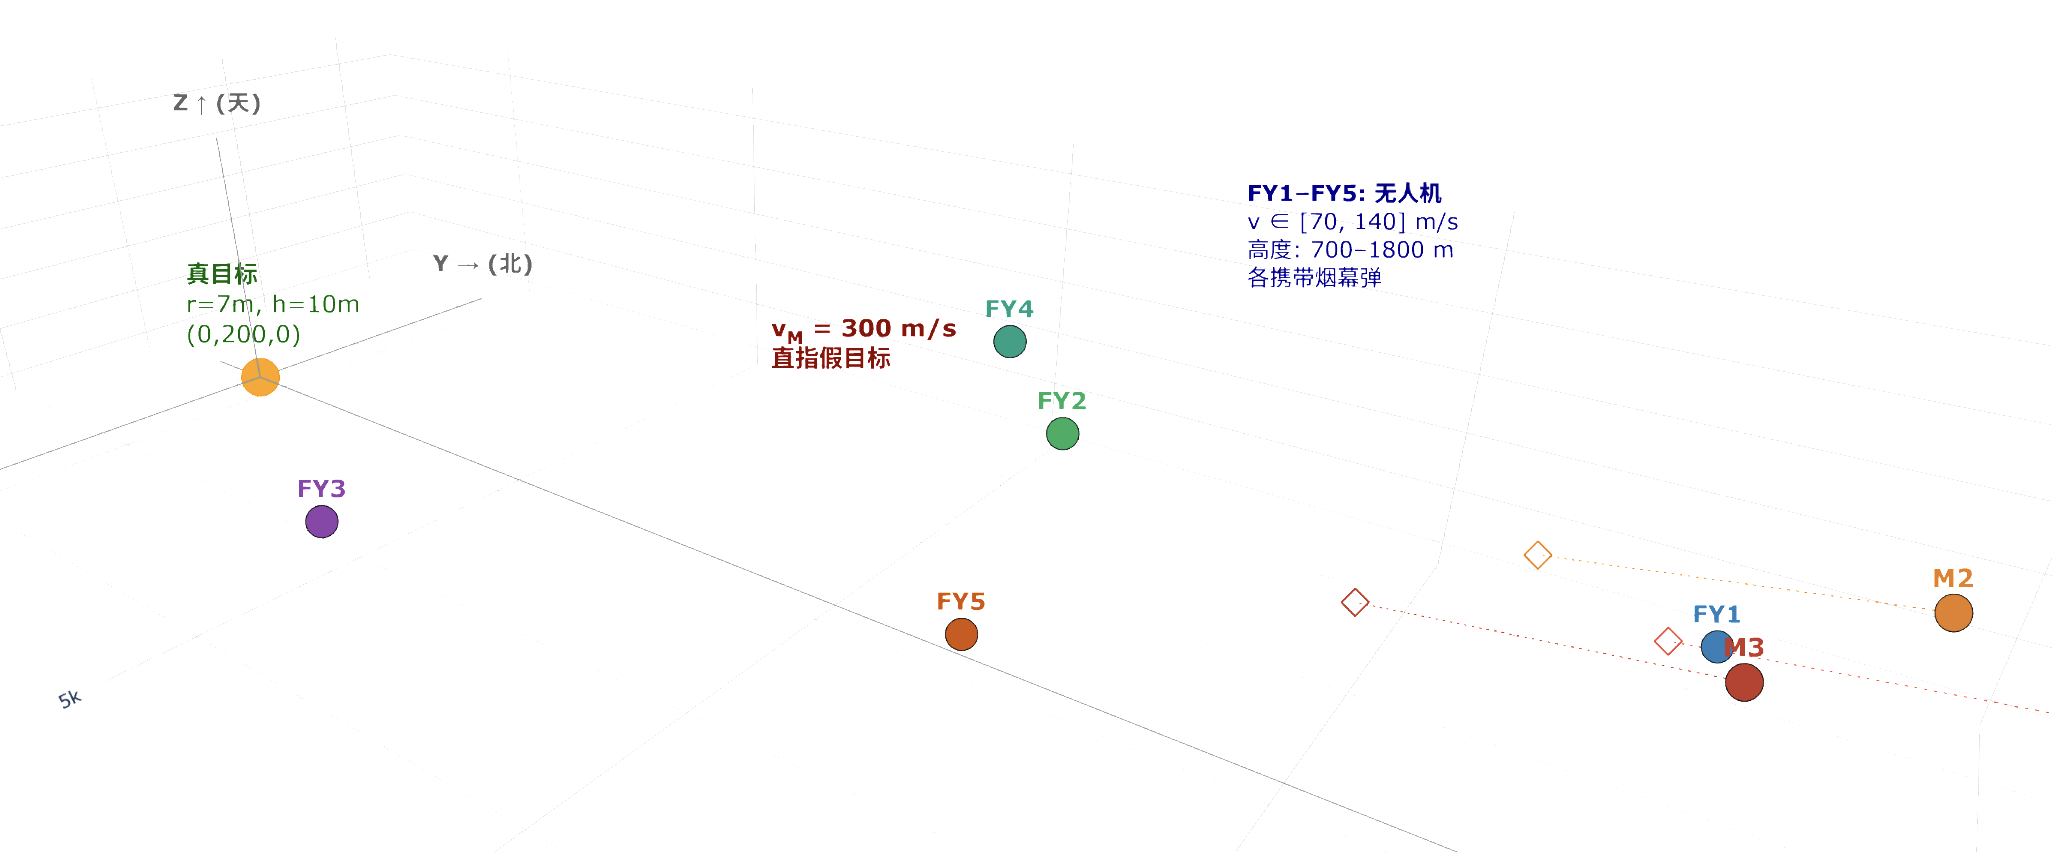
\includegraphics[width=0.8\textwidth]{20260803185247_339_649.png}
    \caption{初始坐标图}
    \label{fig:initial_coords}
\end{figure}
\subsection{遮蔽判断模型}
为了方便理解，我们将遮蔽问题简化为点、球面和圆柱体三者之间的静态位置关系问题。

记导弹所在点为$\mathbf{M}$，起爆后球 $\mathcal{B}$的球心为$\mathbf{A}$，球的张角为$\alpha$，圆柱体 $\mathcal{C}$表面上任意一点为$\mathbf{P}$，则有效遮挡的情形如下图所示：

\begin{figure}[H]
    \centering
    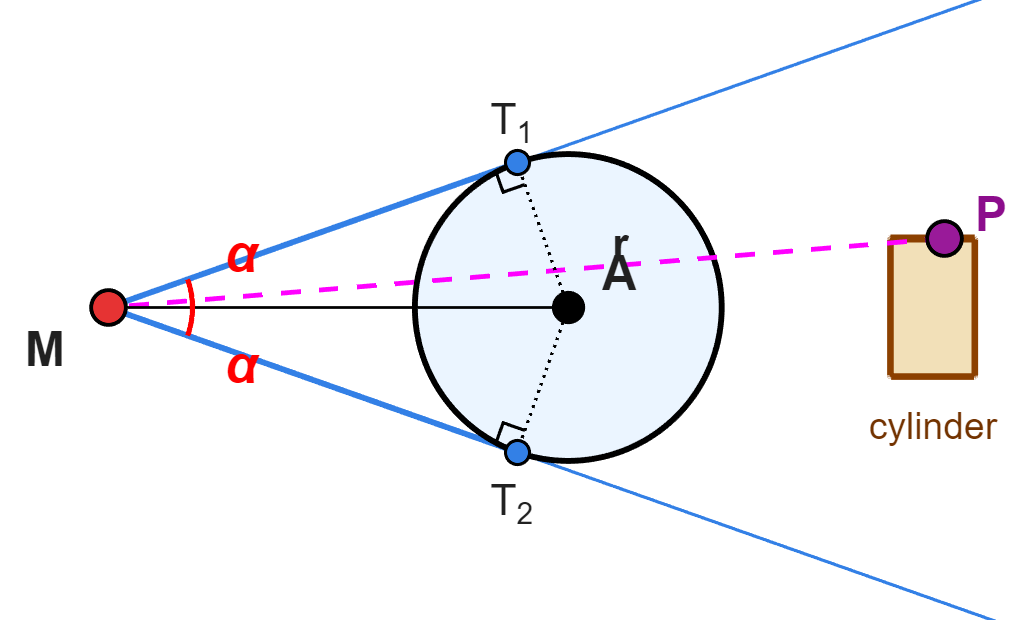
\includegraphics[width=0.8\textwidth]{20260803193802_233_32.png}
    \caption{有效遮挡情况}
    \label{fig:effective_shielding}
\end{figure}
\subsubsection{单位球面映射}
若我们在导弹的位置向量$\mathbf{M}$处作一个单位球面 $\mathbb{S}^2$，我们模拟光线的成像，将圆柱形的轮廓和烟幕球的轮廓均逆着视线的方向投影到$ \mathbb{S}^2$上。如此，我们仅需关注视线的方向，无需关注视线的长度。若这个点为点$P$，则其投影到这个单位球面后的单位向量为
\[
\pi_{\mathbf{M}}(\mathbf{P}) = \frac{\mathbf{P} - \mathbf{M}}{\|\mathbf{P} - \mathbf{M}\|}, \quad \mathbf{P} \neq \mathbf{M}.
\]
\subsubsection{圆柱面的投影}
如果我们从斜上方观察圆柱体的轮廓，我们发现其轮廓可以由四条线组成，从下图可以直观看出：

\begin{figure}[H]
    \centering
    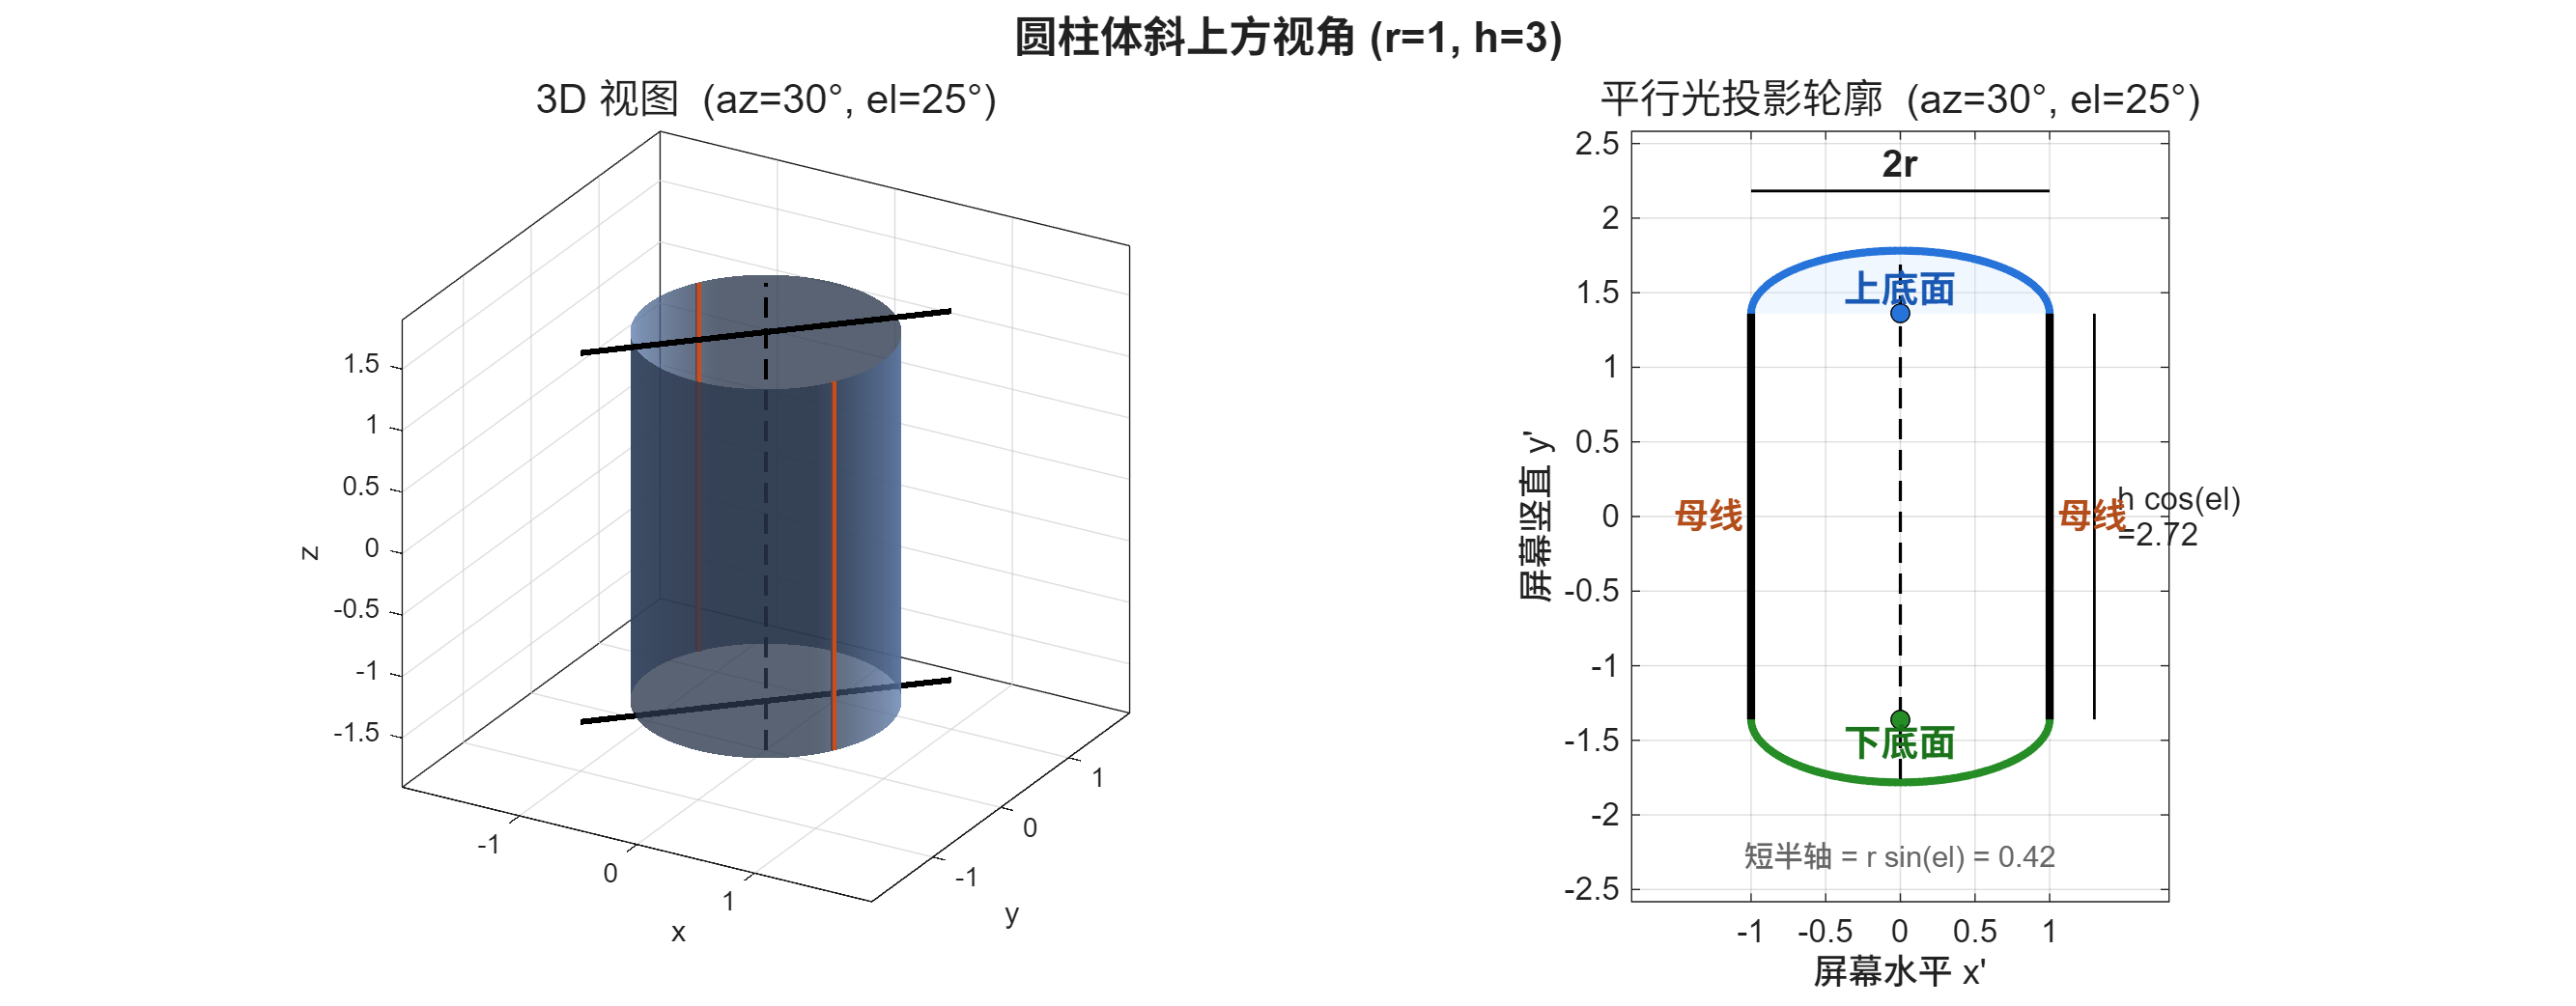
\includegraphics[width=0.8\textwidth]{cylinder_projection.png}
    \caption{圆柱体投影情况}
    \label{fig:cylinder_projection}
\end{figure}


具体如下表所示：
\begin{table}[h]
\centering
\begin{tabular}{c|c|c}
\toprule
边界 & 参数方程 & 说明 \\
\midrule
左切线 $\mathcal{L}_L$ & $\mathbf{T}_L + (0,0,s),\; s\in[0,H]$ & 从 $\mathbf{M}$ 到圆柱的左切线竖线段 \\
右切线 $\mathcal{L}_R$ & $\mathbf{T}_R + (0,0,s),\; s\in[0,H]$ & 右切线竖线段 \\
顶面弧 $\mathcal{E}_{\text{top}}$ & $O_1 + (0,0,H) + r(\cos\phi,\sin\phi,0)$ & 顶面可见椭圆弧 \\
底面弧 $\mathcal{E}_{\text{bot}}$ & $O_1 + r(\cos\phi,\sin\phi,0)$ & 底面可见椭圆弧（远离 $\mathbf{M}$ 的半弧） \\
\bottomrule
\end{tabular}
\end{table}

其中 $\mathbf{T}_L, \mathbf{T}_R$ 是 $\mathbf{M}$ 到圆柱圆周（xy平面）的两切点，切线半角 $\psi = \arcsin(r / d_{xy})$，\\$d_{xy} = \sqrt{(M_x)^2 + (M_y-200)^2}$。\\
圆柱投影区域：
\[
\Omega_{\mathcal{C}}(\mathbf{M}) = \{\pi_{\mathbf{M}}(\mathbf{P}) \mid \mathbf{P} \in \partial\mathcal{C}_{\text{vis}}(\mathbf{M})\}.
\]
实际计算中，对 $\partial\mathcal{C}_{\text{vis}}$ 均匀采样 $N \approx 215$ 个点，得到方向向量集 $\{\mathbf{u}_i\}_{i=1}^{N}$。

\subsubsection{烟幕球投影区域}

烟幕球 $\mathcal{B}(\mathbf{A}, R_s)$ 投影到单位球面上是一个球冠：
\[
\Omega_{\mathcal{B}}(\mathbf{M}, \mathbf{A}) = \left\{\mathbf{u} \in \mathbb{S}^2 \;\middle|\; \arccos(\mathbf{u} \cdot \mathbf{u}_A) \leq \alpha\right\},
\]
其中
\[
\mathbf{u}_A = \pi_{\mathbf{M}}(\mathbf{A}) = \frac{\mathbf{A} - \mathbf{M}}{\|\mathbf{A} - \mathbf{M}\|}, \quad \alpha = \arcsin\left(\frac{R_s}{\|\mathbf{M} - \mathbf{A}\|}\right).
\]
$\mathbf{u}_A$ 为球冠中心方向，$\alpha$ 为球冠半角（烟幕球对 $\mathbf{M}$ 的张角的一半）。

\subsubsection{遮蔽判定}

\begin{definition}
烟幕球 $\mathcal{B}(\mathbf{A}, R_s)$ 完全遮挡圆柱体 $\mathcal{C}$，当且仅当圆柱体的投影区域被烟幕球的投影球冠完全包含，即：
\[
\Omega_{\mathcal{C}}(\mathbf{M}) \subseteq \Omega_{\mathcal{B}}(\mathbf{M}, \mathbf{A}).
\]
\end{definition}
此时情况如下图所示（为方便查看，此处画的并非单位圆）

\begin{figure}[H]
    \centering
    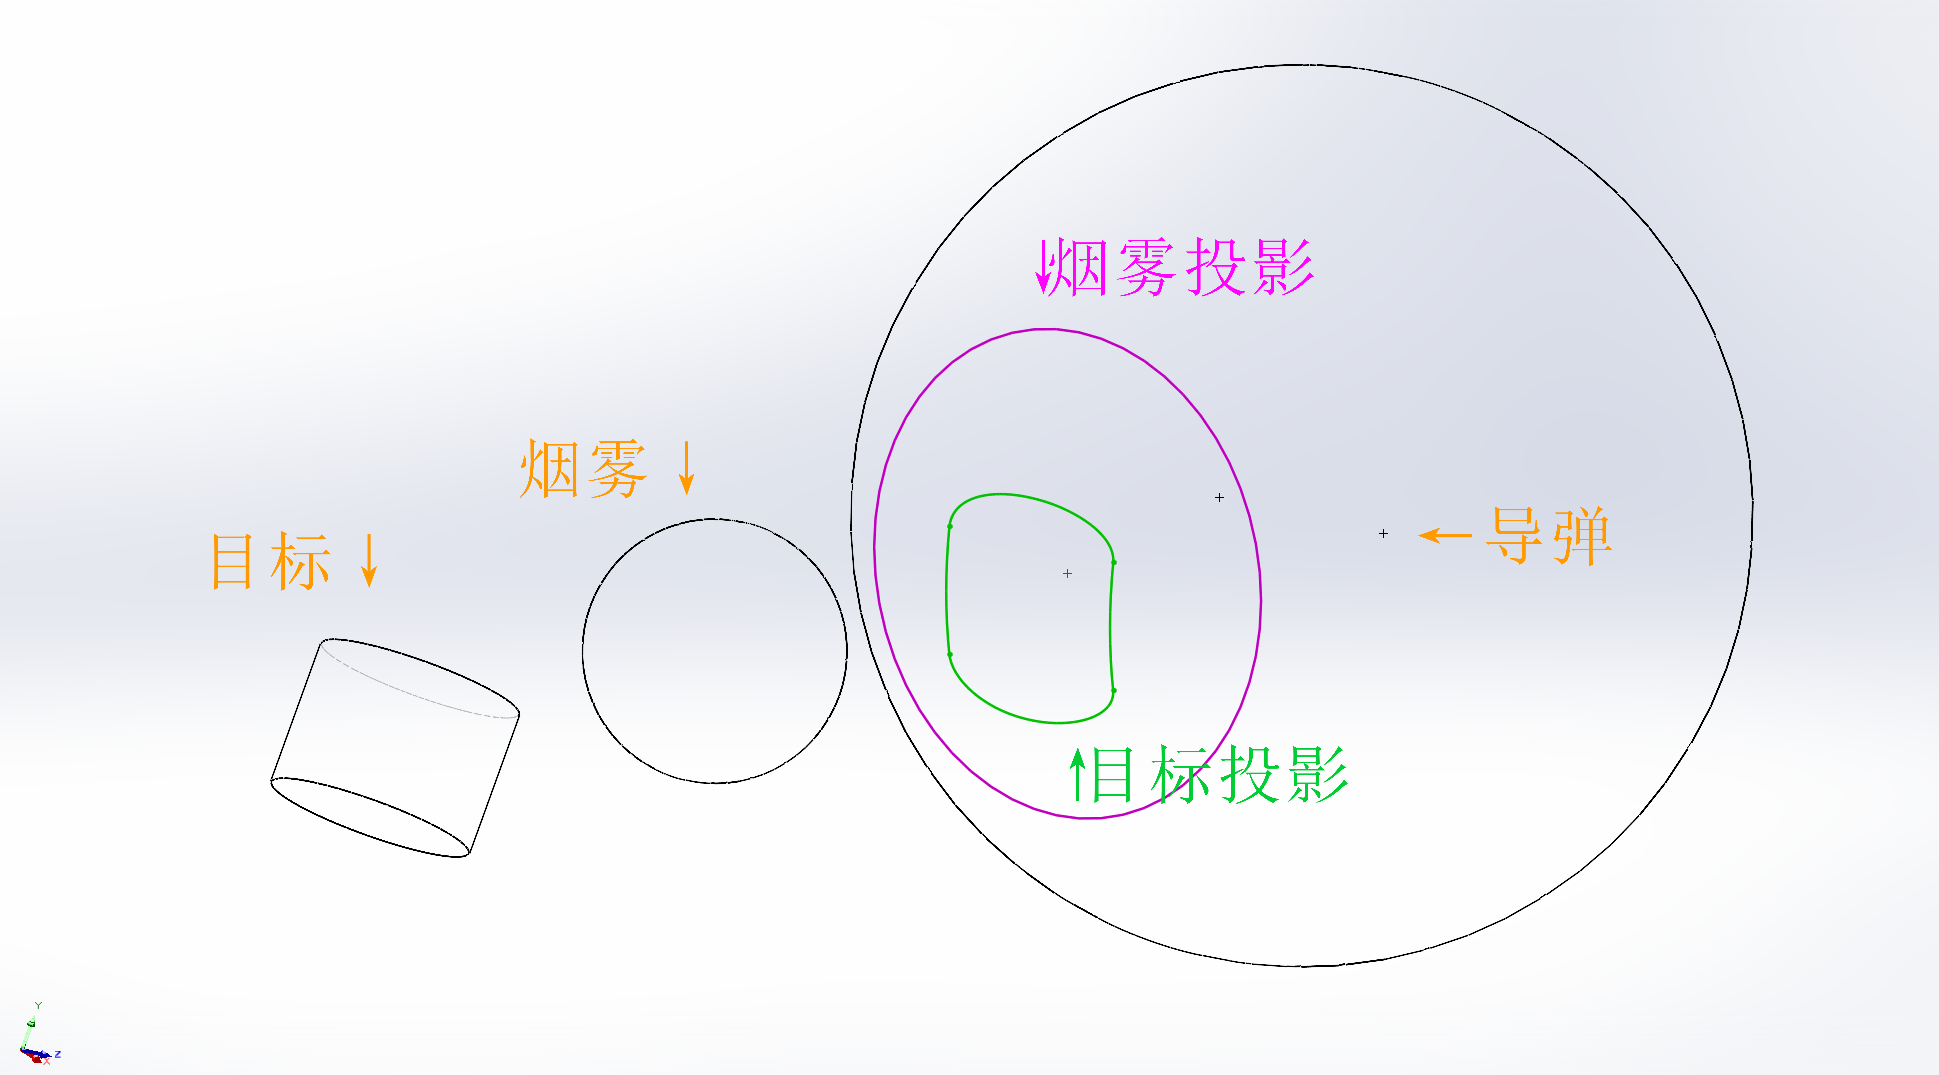
\includegraphics[width=0.8\textwidth]{20260803163444_333_649.png}
    \caption{完全遮蔽投影情况}
    \label{fig:complete_shielding}
\end{figure}
\subsubsection{有效遮蔽约束}
\textbf{情况一：}

当导弹在烟幕球内部时，遮蔽自然有效：
\[
\|\mathbf{M} - \mathbf{A}\| \leq R_s.
\]

我们将该条件称作\textbf{条件C1}

\textbf{情况二：}

当导弹在烟幕球外部，即$\|\mathbf{M} - \mathbf{A}\| > R_s$ 时，需要以下两个条件均满足方能达成遮蔽：

\textbf{条件a — 烟幕位于导弹与目标之间}：
\[
\|\mathbf{M} - O_1\| > \|\mathbf{A} - O_1\|,
\]


\textbf{条件b — 圆柱投影 $\subseteq$ 球冠投影}：
\[
\max_{\mathbf{u} \in \Omega_{\mathcal{C}}(\mathbf{M})} \arccos(\mathbf{u} \cdot \mathbf{u}_A) \leq \arcsin\left(\frac{R_s}{\|\mathbf{M} - \mathbf{A}\|}\right).
\]
即圆柱投影区域中，距离球冠中心 $\mathbf{u}_A$ 最远的方向向量，其角距离不超过球冠半角 $\alpha$。

等价地，定义
\[
\theta_{\max}(\mathbf{M}, \mathbf{A}) \triangleq \max_{\mathbf{P} \in \partial\mathcal{C}_{\text{vis}}(\mathbf{M})} \arccos\left(\frac{(\mathbf{P}-\mathbf{M}) \cdot (\mathbf{A}-\mathbf{M})}{\|\mathbf{P}-\mathbf{M}\| \cdot \|\mathbf{A}-\mathbf{M}\|}\right),
\]
则条件b可写为
\[
\theta_{\max}(\mathbf{M}, \mathbf{A}) \leq \arcsin\left(\frac{R_s}{\|\mathbf{M}-\mathbf{A}\|}\right).
\]

我们将条件a和b称为\textbf{条件C2}

\textbf{总结}：
我们总结一下上述所有不等式，并考虑球心和导弹位置随时间的变化情况，将遮挡情况用布尔值表示，得出最终的判别式，则有：
\begin{equation}
\text{Shielded}(t) = \begin{cases}
True, & \|\mathbf{M}(t) - \mathbf{A}(t)\| \leq R_s \\[6pt]
True, & \begin{aligned}
&\|\mathbf{M}(t) - O_1\| > \|\mathbf{A}(t)- O_1\| \;\land \\
&\|\mathbf{M}(t) - \mathbf{A}(t)\| > R_s \;\land \\
&\theta_{\max}(\mathbf{M}(t), \mathbf{A}(t)) \leq \arcsin\left(\frac{R_s}{\|\mathbf{M}(t) - \mathbf{A}(t)\|}\right)
\end{aligned} \\[6pt]
False, & \text{其他}
\end{cases}
\end{equation}

\section{问题一求解}
根据题意，我们可以画出问题一的空间轨迹和遮蔽关系图：
\begin{figure}[H]
    \centering
    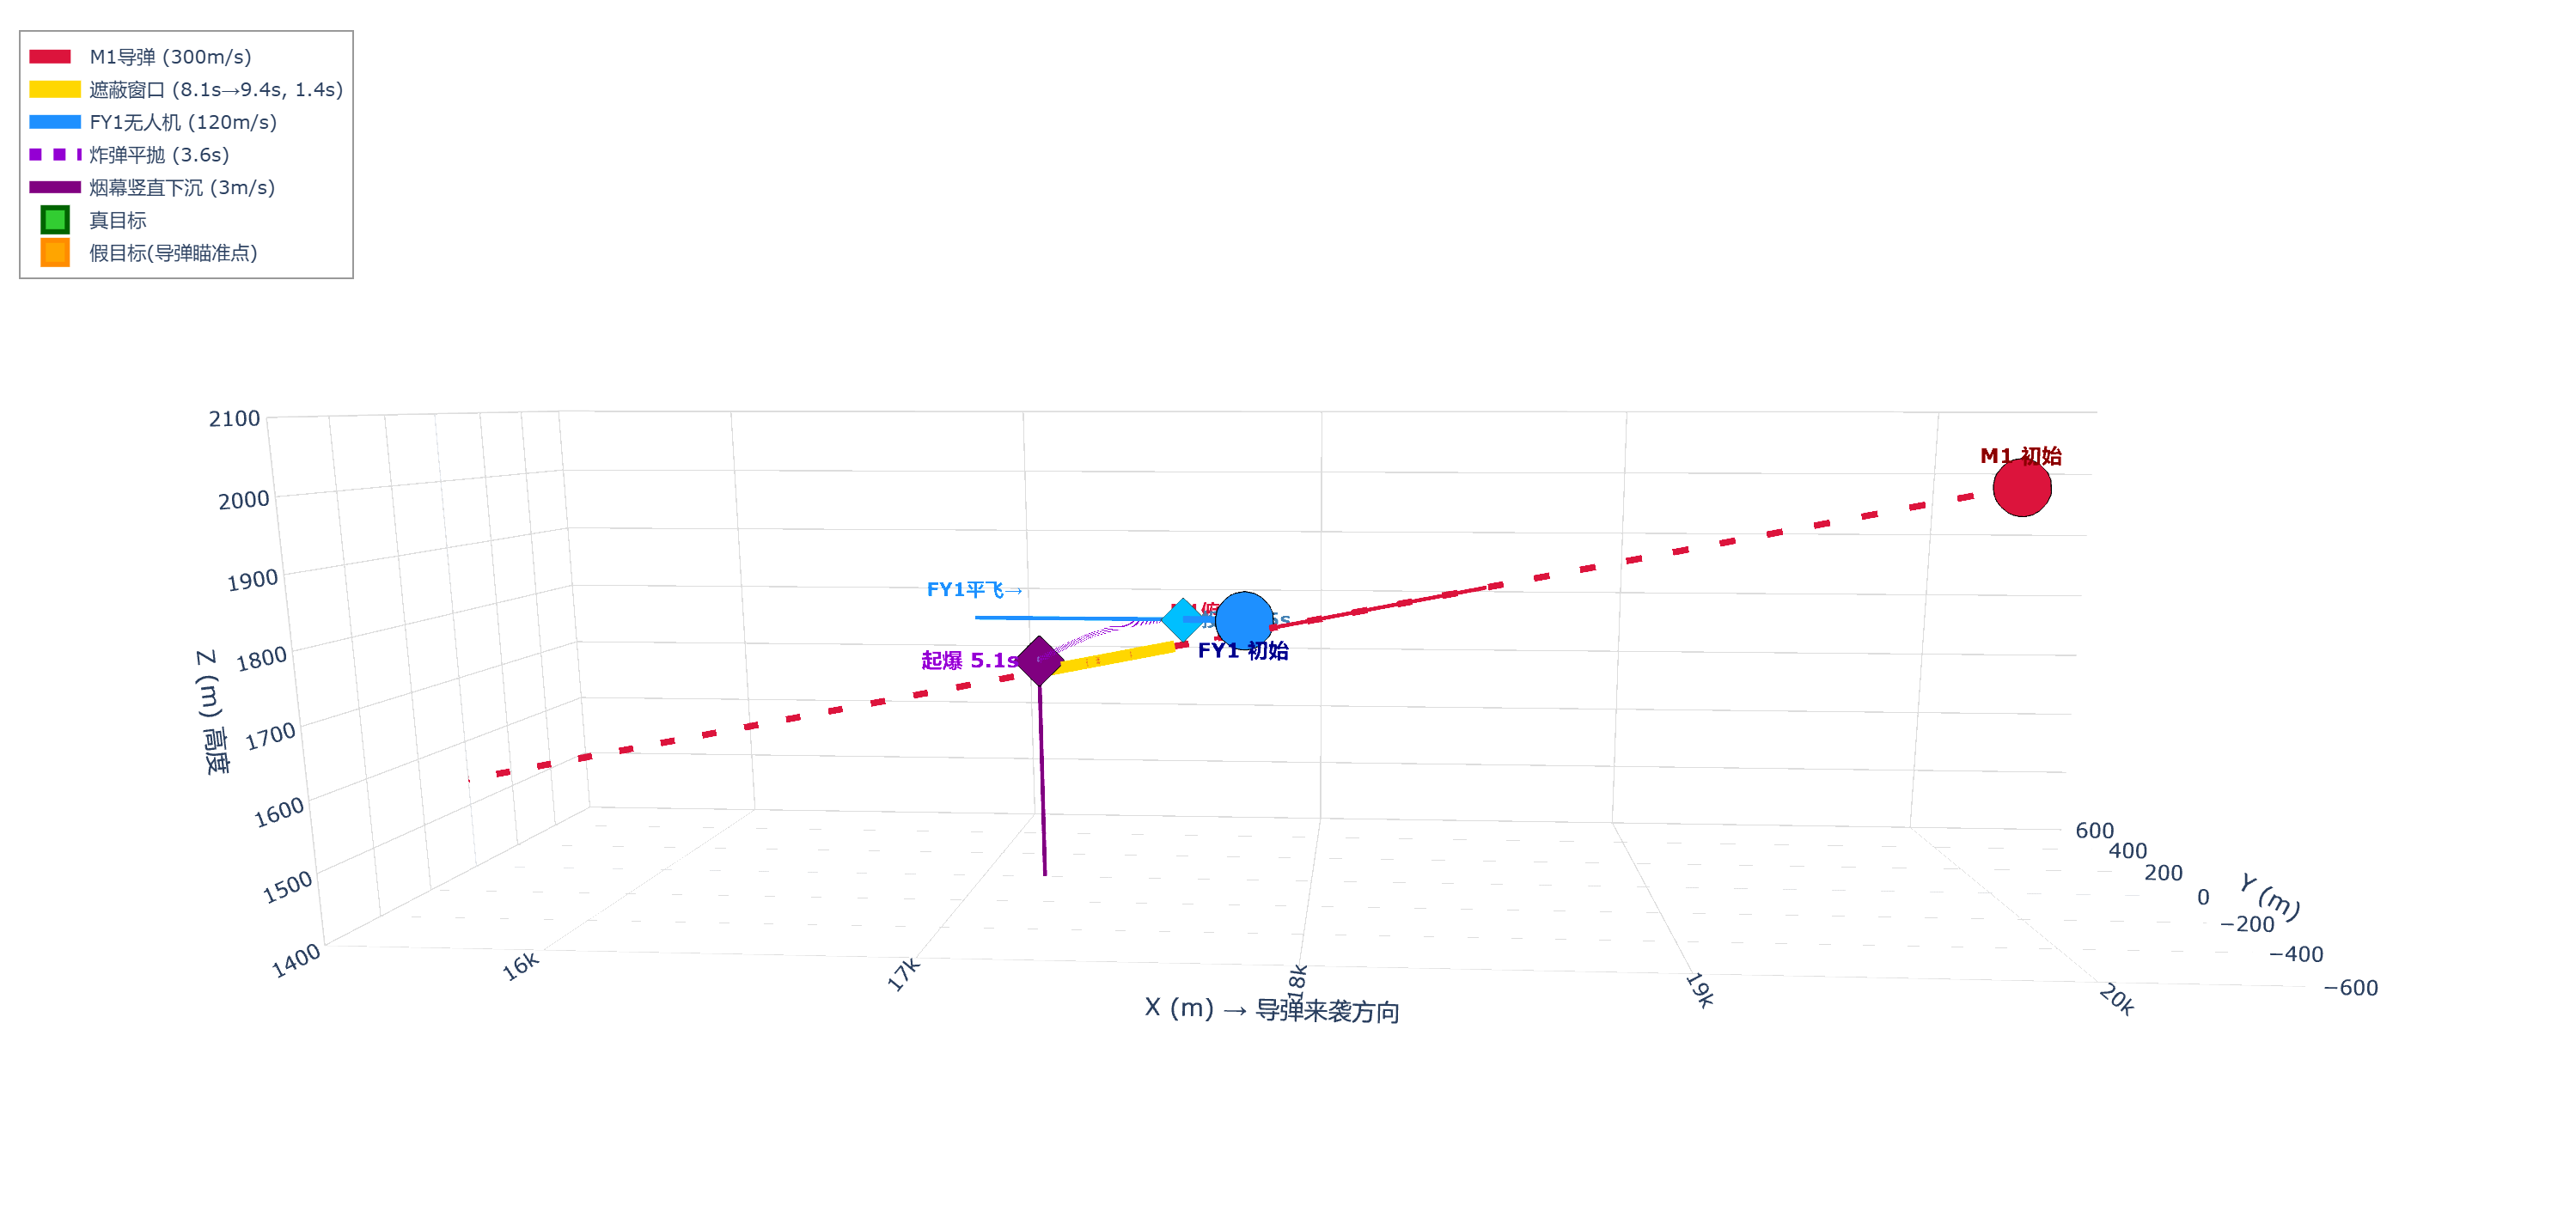
\includegraphics[width=0.8\textwidth]{20260804135851_234_32.png}
    \caption{空间轨迹和遮蔽关系}
    \label{fig:trace}
\end{figure}
\subsection{运动学模型}
\subsubsection{导弹运动方程}
导弹$M_1$初始位置$\mathbf{M}_0=(20000,0,2000)$，其速度恒定为$V_M=300\mathrm{m/s}$，且据题意，该导弹飞行方向不变，沿直线指向原点$O_d$，故其运动为匀速直线运动，运动方向的单位向量为
\[
\hat{\mathbf{u}}_m = \frac{\mathbf{O}_d - \mathbf{M}_0}{\|\mathbf{O}_d - \mathbf{M}_0\|}
= \frac{(-20000, 0, -2000)}{\sqrt{20000^2 + 2000^2}} \approx (-0.995, 0, -0.100)
\]
所以导弹的运动方程以矢量形式可表示为：
\[
\mathbf{M}(t) = \mathbf{M}_0 + \hat{\mathbf{u}}_m \cdot V_M \cdot t
\]
导弹从初始位置飞到原点需时 $T_{\text{end}} = \|\mathbf{M}_0\| / V_M = \sqrt{20000^2 + 2000^2}/300 \approx 67.1\ \mathrm{s}$。
\subsubsection{无人机与烟幕弹}
无人机$FY1$的初始位置为$\mathbf{P}_{\text{FY1}}=(17800,0,1800)$，其以恒定速度$V_{\text{drone}}=120\mathrm{m/s}$朝假目标方向做高度不变的匀速直线运动，若取该方向方向向量$\hat{\mathbf{u}}_f = (-1, 0, 0)$，受领任务后$t_{\text{rel}} = 1.5\ \mathrm{s}$ 时刻投放烟幕弹，延时$t_{\text{delay}} = 3.6\ \mathrm{s}$ 后起爆。

炸弹投放后，由于惯性在水平方向做匀速直线运动，竖直方向受重力作用做匀加速直线运动，我们取 $g = 9.8\ \mathrm{m/s^2}$ 。投放点 $\mathbf{R}_{\text{pt}}$与起爆点 $\mathbf{A}_{\text{det}}$ 的位置可以由矢量形式写为：
\[
\mathbf{R}_{\text{pt}} = \mathbf{P}_{\text{FY1}} + V_{\text{drone}} \cdot \hat{\mathbf{u}}_f \cdot t_{\text{rel}}
\]

故$\mathbf{R}_\text{pt}= (17620, 0, 1800) $
\[
\mathbf{A}_{\text{det}} = \mathbf{R}_{\text{pt}} + V_{\text{drone}} \cdot \hat{\mathbf{u}}_f \cdot t_{\text{delay}} + (0, 0, -\tfrac{1}{2} g t_{\text{delay}}^2)
\]

代入得 $\mathbf{A}_{\text{det}} = (17188, 0, 1736.5)$。

随后，烟幕弹起爆，瞬间形成一个半径$R_s=10\mathrm{m}$的球体，并以$v_s=3\mathrm{m/s}$匀速下沉，其烟幕有效遮蔽时间$T_\text{life}=20\mathrm{s}$。

起爆时刻 $t_{\text{det}} = t_{\text{rel}} + t_{\text{delay}} = 5.1\ \mathrm{s}$。烟幕球心位置的时间函数为：
\[
\mathbf{A}(t) = \mathbf{A}_{\text{det}} - (0, 0, v_s) \cdot (t - t_{\text{det}}), \quad t \in [t_{\text{det}},\; t_{\text{det}}+ T_{\text{life}}].
\]
$t < t_{\text{det}}$ 时烟幕尚未起爆，$t > t_{\text{det}} + T_{\text{life}}$ 时烟幕已失效。所以我们的目标是计算该固定投放参数下烟幕对 M1 的有效遮蔽总时长 $T_{\text{eff}}$。

为了后续求根方便，将烟幕运动改写为
\[
\mathbf{A}(t) = \tilde{\mathbf{A}}_0 - (0,0,v_s)\,t,\quad \tilde{\mathbf{A}}_0 = \mathbf{A}_{\text{det}} + (0,0,v_s)t_{\text{det}},
\]
同时导弹相对烟幕的相对运动为
\begin{equation}
\mathbf{M}(t)-\mathbf{A}(t)=\mathbf{d}_0 + \mathbf{v}_{\text{rel}}\,t,
\end{equation}
其中
\[
\mathbf{d}_0 = \mathbf{M}_0 - \tilde{\mathbf{A}}_0,\qquad
\mathbf{v}_{\text{rel}} = \hat{\mathbf{u}}_m V_M + (0,0,v_s).
\]

\subsection{遮蔽判定与临界方程}
在模型准备中已经给出了遮蔽状态的判别式(1)，这里将其转化为临界方程以便精确求根。遮蔽状态发生切换的时刻正是以下三类方程取等号的时刻。

\subsubsection{C1 边界：导弹进入/离开烟幕球}
条件 C1 为 $\|\mathbf{M}(t)-\mathbf{A}(t)\| \le R_s$，边界方程为
\[
\|\mathbf{M}(t)-\mathbf{A}(t)\|^2 = R_s^2.
\]

将式$(2)$代入，有
\[
\|\mathbf{v}_{\text{rel}}\|^2 t^2 + 2(\mathbf{d}_0\cdot\mathbf{v}_{\text{rel}}) t +  \|\mathbf{d}_0\|^2 - R_s^2 = 0,
\]

这是一个标准的一元二次方程，我们记$a_2 = \|\mathbf{v}_{\text{rel}}\|^2$，$a_1 = 2(\mathbf{d}_0\cdot\mathbf{v}_{\text{rel}})$，$a_0 = \|\mathbf{d}_0\|^2 - R_s^2$，则方程化为
\[
a_2 t^2 + a_1 t + a_0 = 0,
\]

判别式 $\Delta = a_1^2 - 4a_2a_0$，当 $\Delta\ge 0$ 时两根为
\[
t_{\text{enter}},\;t_{\text{exit}} = \frac{-a_1 \mp \sqrt{\Delta}}{2a_2}.
\]

我们保留落在有效区间 $[t_{\text{det}}, t_{\text{det}}+T_{\text{life}}]$ 内的根，这就是导弹进入烟幕球和离开烟幕球的精确时刻。

\subsubsection{C2 边界}
C2 条件包含两个子条件：角度覆盖（条件b）和几何前置（条件a）。故对其边界分别处理。

\textbf{条件b边界}：
定义函数
\[
f_{\text{C2}}(t) = \alpha(t) - \theta_{\max}(t),
\]
其中$\alpha(t)$与$\theta_{\max}(t)$均为模型准备中定义的函数：
\[
\alpha(t)=\arcsin\!\left(\frac{R_s}{\|\mathbf{M}(t)-\mathbf{A}(t)\|}\right),
\]
\[
\theta_{\max}(t)=\max_{\mathbf{P}\in\partial\mathcal{C}_{\text{vis}}(\mathbf{M}(t))}
\arccos\!\left(
\frac{(\mathbf{P}-\mathbf{M}(t))\cdot(\mathbf{A}(t)-\mathbf{M}(t))}
{\|\mathbf{P}-\mathbf{M}(t)\|\,\|\mathbf{A}(t)-\mathbf{M}(t)\|}
\right).
\]
$f_{\text{C2}}(t)>0$ 表示角度覆盖成立。由于我们无法计算出 $f_{\text{C2}}(t)=0$的一个精确解析解，所以我们采用二分法来数值计算。具体步骤：
\begin{enumerate}
    \item 在 $[t_{\text{det}}, t_{\text{det}}+T_{\text{life}}]$ 上均匀取 40 个点，步长 $0.5\mathrm{s}$，计算 $f_{\text{C2}}$。
    \item 若相邻点函数值异号，则在该小区间内用二分法求根，精度设为 $10^{-6}\mathrm{s}$。
\end{enumerate}

\textbf{条件a边界}：
当导弹和烟幕球心与真目标等距时，C2失效，即
\[
\|\mathbf{M}(t)-O_1\|^2 = \|\mathbf{A}(t)-O_1\|^2.
\]

同样代入运动方程，整理为二次方程
\[
a_2^g t^2 + a_1^g t + a_0^g = 0,
\]

其中
\[
a_2^g = \|\hat{\mathbf{u}}_m V_M\|^2 - v_s^2,\quad
a_1^g = 2\big[(\mathbf{M}_0-O_1)\cdot(\hat{\mathbf{u}}_m V_M) + (\tilde{\mathbf{A}}_0-O_1)\cdot(0,0,v_s)\big],
\]
\[
a_0^g = \|\mathbf{M}_0-O_1\|^2 - \|\tilde{\mathbf{A}}_0-O_1\|^2.
\]

取其落在有效区间且满足 $\|\mathbf{M}-O_1\| \le \|\mathbf{A}-O_1\|$ 的根，记为 $t_{\text{geom}}$，该时刻之后烟幕已不再位于目标前方。

\subsection{问题一数值结果}
将问题一给定的参数代入上述方程，求得各临界时刻如下（已舍弃一些不需要的边界条件等）：
\begin{center}
\begin{tabular}{c|c|c|c|c}
\toprule
$t_{\text{det}}$（起爆）& $t_{\text{C2\_start}}$（C2开始）& $t_{\text{C1\_enter}}$（入球）& $t_{\text{geom}}$（几何失效）& $t_{\text{C1\_exit}}$（出球）\\
\midrule
$5.100$ & $8.057$ & $9.388$ & $9.419$ & $9.449$ \\
\bottomrule
\end{tabular}
\end{center}

根据这些临界点，我们可以还原出导弹被遮蔽的全过程：
\begin{itemize}
    \item 起爆后至$8.057$s：$\alpha$不足，无遮蔽。
    \item $8.057$s至$9.388$s：角度覆盖成立（导弹在球外），时长$1.332$s。
    \item $9.388$s至$9.419$s：导弹进入烟幕球内，此时条件C1满足。
    \item $9.419$s至$9.449$s：C2条件失效，但C1条件满足，此时导弹仍在球内，仍是有效遮蔽。
    \item $9.449$s以后：导弹出球，C1失效，遮蔽结束。
\end{itemize}
因此有效遮蔽总时长
\[
T_{\text{eff}} =9.449-8.057= 1.392\ \mathrm{s}.
\]

该时长仅占导弹全程飞行时间$67.1$s的约$2.1\%$，表明在给定的固定参数下遮蔽效果十分有限，这也凸显了后续问题中开展参数优化的必要性。
\section{问题二求解}

问题二在问题一的基础上，将无人机航向、速度、烟幕弹投放与起爆时机作为决策变量，以最大化有效遮蔽时间 $T_{\text{eff}}$ 为目标，建立单机单弹策略优化模型。由于目标函数无解析梯度，可行域在四维空间中极为狭窄，传统梯度方法与全局随机搜索均难以奏效，我们采用\textbf{锚点搜索 + 局部贝叶斯优化（BO）}的两阶段策略进行求解。

\subsection{决策变量与约束条件}

根据问题一，烟幕弹的投放与起爆过程可由起爆时刻 $t_{\text{det}}$ 和起爆点 $\mathbf{A}_{\text{det}}=(A_x,A_y,A_z)$ 唯一确定。而无人机飞行速度可以由起爆点与起点的水平距离反推，投放时刻则可由起爆时刻减去自由落体时间得到。定义四维决策向量为
\[
\mathbf{x} = [\,t_{\text{det}},\; A_x,\; A_y,\; A_z\,] \in \mathbb{R}^4.
\]

给定 $\mathbf{x}$ 后，无人机飞行参数由以下逆向公式唯一确定：
\begin{align}
v(\mathbf{x}) &= \frac{\sqrt{(A_x - 17800)^2 + (A_y)^2}}{t_{\text{det}}}, \label{eq:v_rev} \\
t_{\text{fall}}(\mathbf{x}) &= \sqrt{\frac{2(1800 - A_z)}{g}}, \quad g = 9.8\ \mathrm{m/s^2}, \\
t_{\text{rel}}(\mathbf{x}) &= t_{\text{det}} - t_{\text{fall}}.
\end{align}

约束条件包括：
\begin{enumerate}
    \item \textbf{速度限制}：$v \in [70, 140]\ \mathrm{m/s}$；
    \item \textbf{投放时刻非负}：$t_{\text{rel}} \geq 0$；
    \item \textbf{起爆高度合理}：$A_z \in [50, 1795]\ \mathrm{m}$。
\end{enumerate}

目标函数 $T_{\text{eff}}(\mathbf{x})$ 沿用问题一的遮蔽判定模型，每次评估需计算圆柱投影、二分求根等步骤，耗时约 $0.1\mathrm{s}$。

\subsection{可行域稀疏性与锚点搜索}

在正式执行贝叶斯优化之前，我们首先通过 $5000$ 次随机采样验证了可行域的稀疏性。在搜索空间内均匀采样，结果发现满足所有约束且 $T_{\text{eff}}>0$ 的命中率为 $0/5000=0\%$。其物理原因是：烟幕球心方向必须极其精确地对准圆柱体方向，偏离角度稍微偏一点点则无法遮蔽。所以，可行域应是四维空间中的一个“针尖”状极窄区域，因此从零开始的全局贝叶斯优化必然失败，高斯过程在绝大多数采样点上只观测到常数 $T_{\text{eff}}\approx 0$，无法学到空间结构。

为此，我们采用两阶段优化策略：第一阶段通过“粗粒度网格 + Nelder-Mead 精化”的组合方法定位一个已知可行且较优的解作为锚点；第二阶段以锚点为中心划定局部搜索框，在框内用高斯过程代理模型与期望改进采集函数进行精细优化。

\subsubsection{粗粒度网格遍历}
由起爆点应位于无人机起点附近、导弹飞行路径沿线，且根据问题一中已知的较优解（$\mathbf{x}=[2.80, 17603, 5, 1765]$，$T_{\text{eff}}\approx 4.51\ \mathrm{s}$），我们确定搜索范围如下：
\[
t_{\text{det}} \in [2.0, 4.3]\ \mathrm{s},\quad A_x \in [17550, 17700]\ \mathrm{m},\quad A_y \in [-15, 15]\ \mathrm{m},\quad A_z \in [1740, 1790]\ \mathrm{m}.
\]

我们在四维欧几里得空间中进行“直线网分割”，取各维区间长度 $6$ 等分，我们得到了共 $6^4=1296$ 个节点。网格遍历算法对每个节点调用可行性检查，仅对可行点调用完整的 $T_{\text{eff}}$ 计算。在 $1296$ 个节点中，可行点约占 $15\%\sim20\%$。

最终，我们得到网格搜索的最终输出为：
\[
\mathbf{x}_{\text{grid}} = [t_{\text{det}} = 2.86,\; A_x = 17610,\; A_y = 3,\; A_z = 1770], \quad T_{\text{eff}} = 4.5111\ \mathrm{s}.
\]

\subsubsection{Nelder-Mead 局部精化}
在初步缩小了网格搜索的范围后，我们对这一结果进行“细调”。我们以网格最优解为中心，采用 Nelder-Mead 单纯形法进行无梯度局部精化，使单纯形向目标函数的极小值方向移动。初始单纯形其余四个顶点分别在各维增加小扰动步长 $[0.02, 20, 3, 8]$（这分别对应了 $t_{\text{det}}, A_x, A_y, A_z$ 的数量级）。

然而，由于“针尖”可行域附近的目标函数曲面极度陡峭，NM 的单纯形容易在操作中跳出可行域，导致 $T_{\text{eff}}$ 虚高。为克服这一问题，我们决定，当 NM 结果超过参考值 $4.5064\ \mathrm{s}$ 的 $3\%$时，我们就让其回退至参考值 $\mathbf{x}_{\text{ref}} = [2.80, 17603, 5, 1765]$。

最终，我们得到的精化后的锚点为：
\[
\mathbf{x}_{\text{anchor}} = [t_{\text{det}} = 2.80,\; A_x = 17603,\; A_y = 5,\; A_z = 1765], \quad T_{\text{eff}} = 4.5064\ \mathrm{s}.
\]

我们将其代入公式(3)(4)(5)，反推无人机飞行参数：
\[
v \approx 70.4\ \mathrm{m/s},\quad \theta \approx 178.5^\circ,\quad t_{\text{fall}} \approx 2.67\ \mathrm{s},\quad t_{\text{rel}} \approx 0.13\ \mathrm{s}.
\]


\subsection{高斯过程}
贝叶斯优化的第一步是选取 $n_0=30$ 个初始点并真实计算其 $T_{\text{eff}}$ 值，以建立初始高斯过程代理模型。采样策略采用拉丁超立方采样（LHS），保证各维度的边际覆盖均匀，避免纯随机采样可能出现的扎堆现象。

搜索框以锚点为中心划定：
\[
\mathbf{lb} = [0.5,\; 17303,\; -195,\; 1465], \qquad
\mathbf{ub} = [5.8,\; 17903,\; 205,\; 1790].
\]

高斯过程的核心假设为“相似的起爆策略产生相似的遮蔽时长”，由径向基核函数（RBF）编码：
\[
k(\mathbf{x}, \mathbf{x}') = \sigma_f^2 \exp\!\left(-\frac{1}{2}\sum_{j=1}^{4} \frac{(x_j - x'_j)^2}{\ell_j^2}\right), \label{eq:rbf}
\]
其中 $\ell_j = 0.2 \times (ub_j - lb_j)$ 为各维长度尺度，$\sigma_f^2 = 2.0$ 为信号方差，对应 $T_{\text{eff}}$ 的典型范围。

设已有 $n$ 个真实评估点 $(\mathbf{X}, \mathbf{y}) = \{(\mathbf{x}_i, y_i)\}_{i=1}^n$，其中 $y_i = T_{\text{eff}}(\mathbf{x}_i)$（或惩罚值）。构造核矩阵 $\mathbf{K} \in \mathbb{R}^{n\times n}$，$\mathbf{K}_{ij}=k(\mathbf{x}_i,\mathbf{x}_j)$。对于新候选点 $\mathbf{x}_*$，定义核向量 $\mathbf{k}_*$，$(\mathbf{k}_*)_i=k(\mathbf{x}_i,\mathbf{x}_*)$。高斯过程后验分布的均值与方差为：
\[
\mu(\mathbf{x}_*) = \mathbf{k}_*^T (\mathbf{K} + \sigma_n^2 \mathbf{I})^{-1} \mathbf{y}, \qquad
\sigma^2(\mathbf{x}_*) = k(\mathbf{x}_*, \mathbf{x}_*) - \mathbf{k}_*^T (\mathbf{K} + \sigma_n^2 \mathbf{I})^{-1} \mathbf{k}_*, \label{eq:posterior}
\]
其中 $\sigma_n^2 = 10^{-3}$ 为极小的观测噪声项，仅用于保证矩阵数值可逆。

\subsection{期望改进采集函数与约束处理}

高斯过程给出任意候选策略 $\mathbf{x}$ 的预测均值 $\mu(\mathbf{x})$ 和标准差 $\sigma(\mathbf{x})$。设当前已知最优遮蔽时长为 $y_{\text{best}} = \max_i T_{\text{eff}}(\mathbf{x}_i)$，则期望改进（EI）采集函数定义为：
\[
\mathrm{EI}(\mathbf{x}) = \mathbb{E}_{T \sim \mathcal{N}(\mu, \sigma^2)}[\max\{T - y_{\text{best}}, 0\}] = \Delta \cdot \Phi(Z) + \sigma \cdot \phi(Z), \label{eq:ei}
\]
其中
\[
\Delta = \mu(\mathbf{x}) - y_{\text{best}} - \xi, \qquad Z = \frac{\Delta}{\sigma(\mathbf{x})},
\]
$\xi = 0.01$ 为探索偏置参数，$\Phi,\phi$ 分别为标准正态分布的累积分布函数与概率密度函数。EI 的两项分别对应利用（在已知高值区域附近精调）与探索（在未充分探测的区域冒险），其自适应平衡是贝叶斯优化高效收敛的关键。

对于不可行策略，若直接返回 $T_{\text{eff}}=0$，高斯过程将在可行域边界处观测到从正值到零的“悬崖”，建模质量极差。我们采用\textbf{平滑惩罚法}：将各约束违反量连续归一化后求和作为惩罚值，对不可行策略返回负惩罚：
\[
y(\mathbf{x}) = \begin{cases}
T_{\text{eff}}(\mathbf{x}), & \text{若 } \mathbf{x} \text{ 可行}, \\[6pt]
-\operatorname{penalty}(\mathbf{x}), & \text{否则}.
\end{cases}
\]
惩罚函数包含速度、高度、投放时刻三项归一化违反量之和。高斯过程在惩罚曲面上能学到连续的梯度，自然地将搜索从不可行区域引导至可行域边界。

\subsection{优化算法流程与结果}

完整的局部贝叶斯优化算法流程如下：

\textbf{步骤1：} 用拉丁超立方采样生成 $n_0=30$ 个初始点，注入已知锚点 $\mathbf{x}_{\text{anchor}}$，计算对应的 $T_{\text{eff}}$ 值。

\textbf{步骤2：} 循环执行 $N=120$ 次：
\begin{enumerate}
    \item 训练高斯过程模型，得到所有候选点的预测均值 $\mu$ 和标准差 $\sigma$；
    \item 随机生成 $30000$ 个候选策略，计算各自的 $\mathrm{EI}$ 值，选取最大的 $\mathbf{x}_{\text{next}}$；
    \item 真实评估 $T_{\text{eff}}(\mathbf{x}_{\text{next}})$，更新数据集；
    \item 若 $T_{\text{eff}}(\mathbf{x}_{\text{next}})$ 优于当前最优，则更新最优解。
\end{enumerate}

\textbf{步骤3：} 返回最优策略及相应的遮蔽时长。

超参数配置：初始点 $n_0=30$，BO 迭代 $N=120$（累计 $150$ 次评估），RBF核长度尺度 $\ell_j=0.2(ub_j-lb_j)$，信号方差 $\sigma_f^2=2.0$，噪声 $\sigma_n^2=10^{-3}$，探索偏置 $\xi=0.01$，候选点数量 $M=30000$。

\subsubsection{实验结果}

\textbf{实验1（局部BO）：} 以锚点为中心的局部搜索框内，经 $150$ 次评估收敛，最终结果为：
\[
\mathbf{x}^*_{\text{BO}} = [t_{\text{det}} = 2.80,\; A_x = 17603,\; A_y = 5,\; A_z = 1765], \quad T_{\text{eff}}^* = 4.5064\ \mathrm{s}.
\]

可以看到这个结果与Nelder-Mead 局部精化的结果完全一致，说明其实Nelder-Mead 局部精化已经收敛到最优解。

我们将这个结果代入公式(3)(4)(5)，可得无人机飞行参数：
\begin{align*}
v &= \frac{\sqrt{(17603-17800)^2 + 5^2}}{2.80} \approx 70.4\ \mathrm{m/s}, \\
\theta &= \arctan2(5,\; -197) \approx 178.5^\circ, \\
t_{\text{fall}} &\approx 2.67\ \mathrm{s}, \quad t_{\text{rel}} \approx 0.13\ \mathrm{s}.
\end{align*}

所以，我们得到的最优情况是，无人机以约 $70.4\ \mathrm{m/s}$ 的速度、航向角 $178.5^\circ$（几乎沿 $X$ 轴负方向）飞行，起飞后仅 $0.13\ \mathrm{s}$ 即投放炸弹，炸弹经 $2.67\ \mathrm{s}$ 自由落体后在 $(17603,5,1765)$ 起爆。有效遮蔽时长 $4.5064\ \mathrm{s}$，覆盖导弹全程（$67.1\mathrm{s}$）的约 $6.7\%$。

\textbf{实验2（扩大搜索范围）：} 将搜索框扩展至 $\mathbf{lb}=[0.5,16800,-300,1000]$，$\mathbf{ub}=[10.0,17800,300,1790]$，$150$ 次评估后收敛到相同结果（$T_{\text{eff}}=4.5064\ \mathrm{s}$），说明锚点所在区域确为全局最优，在更大范围内不存在显著更优的配置。

\textbf{实验3（多起点BO）：} 在局部搜索框内以 5 个不同随机种子各运行 BO（$n_0=25$，$N=80$），全部收敛到 $T_{\text{eff}} = 4.5064\ \mathrm{s}$，标准差为 $0$，证明在该局部区域内 BO 的收敛是稳定、确定、非偶然的。

\subsubsection{收敛性分析}

贝叶斯优化不依赖目标函数值的变化判断收敛，而是观察 EI 值随迭代次数的衰减趋势。在实验1中：

\begin{center}
\begin{tabular}{c|c|p{5.5cm}}
\toprule
\textbf{迭代阶段} & \textbf{EI 值} & \textbf{搜索状态} \\
\midrule
第 1 次    & $\mathrm{EI} \approx 0.3$   & GP 从 LHS 学到可行性结构，存在高价值待探索区域 \\
第 25 次   & $\mathrm{EI} \approx 0.05$  & 找到优质区域，在其附近精调（利用主导） \\
第 100--120 次 & $\mathrm{EI} \approx 0.01$  & 搜索框充分覆盖，GP 后验方差趋于 0 \\
\bottomrule
\end{tabular}
\end{center}

当 EI 衰减至 $\sim 0.01$ 且持续下降时，意味着 GP 在搜索框内已处处确定，再增加评估次数几乎不可能提升最优值，算法已收敛。最终得到的 $T_{\text{eff}}=4.5064\ \mathrm{s}$ 较问题一中固定参数的结果 $1.392\ \mathrm{s}$ 提升了约 $224\%$，充分体现了优化策略的有效性。
\section{问题三求解}

问题三在问题二的基础上，将无人机可投放的烟幕弹数量从 1 枚扩展至 3 枚，要求在无人机飞行方向与速度不变的条件下，通过优化三枚弹各自的投放与起爆时机，使总有效遮蔽时间最长。与问题二的核心区别在于：三枚弹共享同一组无人机飞行参数 $(v,\theta)$，其起爆点水平投影共线，无法横向分散部署，只能沿飞行方向前后排布。

\subsection{决策变量与约束条件}

对第 $i$ 枚弹（$i=1,2,3$），投放时刻记为 $t_{\text{rel}}^{(i)}$，起爆延时为 $t_{\text{delay}}^{(i)}$，起爆时刻 $t_{\text{det}}^{(i)} = t_{\text{rel}}^{(i)} + t_{\text{delay}}^{(i)}$。炸弹水平方向继承无人机惯性速度，垂直方向仅受重力。起爆点坐标为
\[
\mathbf{A}^{(i)} = \mathbf{P}_{\text{FY1}} + v \cdot (\cos\theta,\; \sin\theta,\; 0) \cdot t_{\text{det}}^{(i)} + \left(0,\; 0,\; -\frac{1}{2}g\,(t_{\text{delay}}^{(i)})^2\right),
\]
其中 $(A_x^{(i)}, A_y^{(i)})$ 由 $(v,\theta,t_{\text{det}}^{(i)})$ 完全确定，$A_z^{(i)}$ 仅由 $t_{\text{delay}}^{(i)}$ 确定。投放时刻由逆向公式导出：
\[
t_{\text{rel}}^{(i)} = t_{\text{det}}^{(i)} - t_{\text{delay}}^{(i)}, \qquad
t_{\text{delay}}^{(i)} = \sqrt{\frac{2(1800 - A_z^{(i)})}{g}}.
\]

$v$ 和 $\theta$ 对三枚弹共享，每弹拥有独立可调的 $t_{\text{det}}^{(i)}$ 和 $t_{\text{delay}}^{(i)}$，共涉及 $2 + 3 \times 2 = 8$ 个独立决策变量：
\begin{equation}
\mathbf{x} = \left[\,v,\; \theta,\; t_{\text{det}}^{(1)},\; t_{\text{delay}}^{(1)},\; t_{\text{det}}^{(2)},\; t_{\text{delay}}^{(2)},\; t_{\text{det}}^{(3)},\; t_{\text{delay}}^{(3)}\,\right] \in \mathbb{R}^8. \label{eq:x3}
\end{equation}

各变量取值范围：$v \in [70, 140]\ \mathrm{m/s}$，$\theta \in [160^\circ, 200^\circ]$，$t_{\text{det}}^{(i)} \in [0.5, 15.0]\ \mathrm{s}$，$t_{\text{delay}}^{(i)} \in [0.05, 6.0]\ \mathrm{s}$。

约束条件包括：
\begin{enumerate}
    \item 速度限制 $v \in [70, 140]\ \mathrm{m/s}$；
    \item 投放时刻非负 $t_{\text{rel}}^{(i)} \geq 0$；
    \item 起爆高度合理 $A_z^{(i)} \in [50, 1795]\ \mathrm{m}$；
    \item 相邻投放间隔 $t_{\text{rel}}^{(i+1)} - t_{\text{rel}}^{(i)} \geq 1.0\ \mathrm{s}$；
    \item 起爆时刻递增 $t_{\text{det}}^{(1)} < t_{\text{det}}^{(2)} < t_{\text{det}}^{(3)}$。
\end{enumerate}

目标函数为三枚弹遮蔽时段的并集总长度，并附加单弹超界惩罚：
\begin{equation}
\mathcal{F}(\mathbf{x}) = \left|\,\bigcup_{i=1}^{3}\;\mathcal{I}^{(i)}(\mathbf{x})\,\right| - \lambda \sum_{i=1}^{3} \max\left(0,\; T_{\text{eff,single}}^{(i)} - T_{\max}\right), \label{eq:obj3}
\end{equation}
其中 $\mathcal{I}^{(i)}(\mathbf{x})$ 为第 $i$ 枚弹的遮蔽区间集合，$T_{\max} = 4.5064\ \mathrm{s}$ 为问题二单弹最优值（严格的物理上界），惩罚系数 $\lambda = 10$。约束处理沿用问题二的平滑惩罚框架。

\subsection{锚点引导的局部贝叶斯优化}

8 维搜索空间中可行解比例极低，直接从零开始的全局 BO 难以奏效。采用锚点引导的局部 BO 策略：以问题二的最优单弹解为基础，构造三弹的合理初始参数作为锚点。

已知问题二最优单弹解：
\[
v = 70.38\ \mathrm{m/s},\quad \theta = 178.55^\circ,\quad t_{\text{det}} = 2.80\ \mathrm{s},\quad t_{\text{delay}} = 2.673\ \mathrm{s},\quad \mathbf{A} = (17603, 5, 1765),\quad T_{\text{eff}} = 4.5064\ \mathrm{s}.
\]

锚点三弹参数设计如下：
\begin{center}
\begin{tabular}{c|c|c|c}
\toprule
\textbf{弹} & $t_{\text{det}}$ (s) & $t_{\text{delay}}$ (s) & $t_{\text{rel}}$ (s) \\
\midrule
1 & 2.800 & 2.673 & 0.127 \\
2 & 4.500 & 3.200 & 1.300 \\
3 & 6.500 & 3.800 & 2.700 \\
\bottomrule
\end{tabular}
\end{center}
弹 1 直接复用 P2 最优解，弹 2、3 紧凑排布于弹 1 的遮蔽窗口尾部，投放间隔分别为 $1.173\ \mathrm{s}$ 和 $1.400\ \mathrm{s}$，均满足最小间隔约束。

搜索框以锚点为中心，各维半宽取参数变化范围的 3 倍，经裁剪至硬约束边界后，搜索框体积约为整个 8D 空间的 $10^{-4}\sim10^{-5}$ 量级。超参数配置：初始 Latin Hypercube 采样 $n_0=40$ 点，对 $t_{\text{det}}$ 三个维度强制执行升序排列，注入锚点；BO 迭代 $N=100$ 次，累计 $140$ 次评估；RBF核长度尺度 $\ell_j = 0.2(ub_j - lb_j)$，信号方差 $\sigma_f^2 = 2.0$，噪声 $\sigma_n^2 = 10^{-3}$，探索偏置 $\xi = 0.01$；每次 EI 最大化在搜索框内随机生成 $40000$ 个候选点。

\subsection{区间并集算法}

三枚弹的遮蔽区间并集由区间合并算法计算。对每枚弹调用 $\operatorname{compute\_T\_eff\_intervals}$ 获得遮蔽区间列表 $\mathcal{I}^{(i)}$，展平后按起点升序排序，顺序扫描合并重叠区间（容差 $\varepsilon = 10^{-6}\ \mathrm{s}$），累加合并后区间长度即得并集总长。算法复杂度 $O(k\log k)$，$k \leq 6$。

\subsection{数值结果与物理分析}

\subsubsection{最优投放策略}

锚点经目标函数评估后得到 $T_{\text{eff}}^{\text{total}} = 5.3791\ \mathrm{s}$，BO 在 $140$ 次评估中未能显著超越该锚点，侧面印证锚点本身已非常接近该约束下的全局最优。

最优策略的无人机飞行参数与问题二完全一致：
\[
\boxed{v = 70.38\ \mathrm{m/s},\quad \theta = 178.55^\circ}
\]
两个独立问题在无人机飞行方向这一核心参数上精确收敛至同一值，说明该航向确为该场景下的最优航向。

三枚弹的详细投放策略：

\begin{center}
\begin{tabular}{c|c|c|c|c|c|c|c}
\toprule
\textbf{弹} & $t_{\text{rel}}$ (s) & $t_{\text{det}}$ (s) & $t_{\text{delay}}$ (s) & $A_x$ (m) & $A_y$ (m) & $A_z$ (m) & 单弹 $T_{\text{eff}}$ (s) \\
\midrule
1 & 0.127 & 2.800 & 2.673 & 17603 & 5.0 & 1765 & 4.5064 \\
2 & 1.300 & 4.500 & 3.200 & 17483 & 8.0 & 1750 & 0.7237 \\
3 & 2.700 & 6.500 & 3.800 & 17343 & 11.6 & 1729 & 1.6043 \\
\bottomrule
\end{tabular}
\end{center}

物理约束验证：弹 1 的单弹 $T_{\text{eff}} = 4.5064\ \mathrm{s}$ 恰好等于 P2 理论上界，弹 2、3 均严格小于该上界；投放间隔满足 $\geq 1.0\ \mathrm{s}$；三弹 $A_z$ 依次递减，匹配导弹飞行后期高度逐渐降低的物理需求。

\subsubsection{遮蔽时段分析}

各弹遮蔽区间：

\begin{center}
\begin{tabular}{c|c|c}
\toprule
\textbf{弹} & \textbf{遮蔽区间} & \textbf{时长} \\
\midrule
1 & $[3.527,\; 8.034]$ & $4.506\ \mathrm{s}$ \\
2 & $[7.711,\; 8.434]$ & $0.724\ \mathrm{s}$ \\
3 & $[7.302,\; 8.906]$ & $1.604\ \mathrm{s}$ \\
\bottomrule
\end{tabular}
\end{center}

三弹并集：
\[
[3.527,\; 8.034] \cup [7.711,\; 8.434] \cup [7.302,\; 8.906] = [3.527,\; 8.906],
\]
\[
T_{\text{eff}}^{\text{total}} = 8.906 - 3.527 = 5.379\ \mathrm{s}.
\]

弹 1 独力承担了主体遮蔽（$4.506\ \mathrm{s}$，占总遮蔽的 $84\%$）；弹 2 的遮蔽窗口与弹 1 尾部高度重叠，独立净贡献极小；弹 3 将遮蔽终点从 $8.034\ \mathrm{s}$ 延伸至 $8.906\ \mathrm{s}$，贡献了约 $0.872\ \mathrm{s}$ 的净增量。三弹分工：弹 1 主力遮蔽，弹 3 末端延伸，弹 2 过渡衔接。

问题三相比问题二提升约 $19.4\%$——弹数增至 3 倍，遮蔽时长仅增加约 $0.87\ \mathrm{s}$，边际回报显著递减。

\subsubsection{物理局限性}

三枚弹未能实现理想的时间接力遮蔽，根本原因在于速度量级的悬殊差异。无人机以 $70.38\ \mathrm{m/s}$ 沿 $X$ 轴负方向飞行，导弹以 $298.5\ \mathrm{m/s}$ 的水平速度分量俯冲，导弹速度约为无人机的 $4.2$ 倍。

三弹起爆时刻跨度为 $3.7\ \mathrm{s}$（$2.80 \to 6.50$），无人机水平位移仅约 $260\ \mathrm{m}$，导弹水平飞行约 $1104\ \mathrm{m}$。烟幕球半径仅 $10\ \mathrm{m}$，导弹穿过三弹起爆点区域仅需约 $0.87\ \mathrm{s}$，空间分散不足以在时间轴上拉开遮蔽窗口。此外，有效起爆时间窗总长仅约 $5\ \mathrm{s}$（$t_{\text{det}} \in [3, 8]$），超出此范围单弹 $T_{\text{eff}} = 0$。弹 1 的 C2 遮蔽起始于 $3.527\ \mathrm{s}$，终止于 $8.034\ \mathrm{s}$，后两枚弹虽能略微拓展终止边界，但无法向前拓展起始边界——遮蔽窗口起点始终由最早的那枚弹决定。

\subsection{结论}

问题三在问题二最优单弹解的基础上，将搜索空间从 4D 扩展至 8D，以 P2 最优解为锚点，利用锚点引导的贝叶斯优化在 $140$ 次评估内确认了最优投放策略。锚点方案本身即给出了可行且近似最优的解——三弹并集总遮蔽时长 $T_{\text{eff}}^{\text{total}} = 5.379\ \mathrm{s}$，约为 P2 单弹结果的 $1.19$ 倍，覆盖导弹全程的约 $8.0\%$。弹 1 直接复用 P2 最优解（占 $84\%$），弹 2 提供过渡衔接，弹 3 实现末端延伸。三弹边际贡献递减的现象揭示了单机直线飞行约束下多弹接力策略的固有物理上限。
\end{document}